\documentclass[twoside,11pt]{article}

%================================ PREAMBLE ==================================

%--------- Packages -----------
\usepackage{fullpage}
\usepackage{amssymb}
\usepackage{amsmath}
\usepackage{amsthm}
\usepackage{latexsym}
\usepackage{graphicx}
\usepackage{wrapfig}
\usepackage{color}
\usepackage{url}
\usepackage{float}
\usepackage{enumitem}
\usepackage{wrapfig}
\usepackage{titlesec}
%\usepackage{algorithm,algorithmic}

%---------- Spacing ----------
\setlength{\parindent}{0pt}
\setlength{\parskip}{3pt}

\setlist[enumerate]{itemsep=0mm}
\titlespacing*{\section}{0pt}{0.6\baselineskip}{\baselineskip}

%---------Definitions----------
\newcommand{\half}{{\textstyle{\frac{1}{2}}}}
\renewcommand{\>}{{\rightarrow}}
\renewcommand{\hat}{\widehat}
\renewcommand{\tilde}{\widetilde}
\newcommand{\grad}{{\nabla}}
%
\newcommand{\argmax}{\textup{\textrm{argmax}}}
\newcommand{\argmin}{\textup{\textrm{argmin}}}
\newcommand{\argsort}{\textup{\textrm{argsort}}}
\newcommand{\sign}{\textup{\textrm{sign}}}
\newcommand{\poly}{\textup{\textrm{poly}}}
\newcommand{\er}{\textup{\textrm{er}}}
\newcommand{\zo}{\textup{\textrm{0-1}}}
\newcommand{\sq}{\textup{\textrm{sq}}}
%
\newcommand{\1}{{\mathbf 1}}
\newcommand{\0}{{\mathbf 0}}
\newcommand{\I}{{\mathbf I}}
\newcommand{\R}{{\mathbb R}}
\newcommand{\Z}{{\mathbb Z}}
\newcommand{\N}{{\mathbb N}}
\renewcommand{\P}{{\mathbf P}}
\newcommand{\E}{{\mathbf E}}
\newcommand{\Var}{{\mathbf{Var}}}
%
\renewcommand{\a}{{\mathbf a}}
\renewcommand{\b}{{\mathbf b}}
\renewcommand{\c}{{\mathbf c}}
\renewcommand{\d}{{\mathbf d}}
\newcommand{\f}{{\mathbf f}}
\renewcommand{\k}{{\mathbf k}}
\newcommand{\p}{{\mathbf p}}
\newcommand{\q}{{\mathbf q}}
\renewcommand{\u}{{\mathbf u}}
\newcommand{\w}{{\mathbf w}}
\newcommand{\x}{{\mathbf x}}
\newcommand{\y}{{\mathbf y}}
%
\newcommand{\A}{{\mathbf A}}
\newcommand{\bC}{{\mathbf C}}
\newcommand{\C}{{\mathcal C}}
\newcommand{\cD}{{\mathcal D}}
\newcommand{\F}{{\mathcal F}}
\renewcommand{\H}{{\mathcal H}}
\newcommand{\K}{{\mathbf K}}
\renewcommand{\L}{{\mathcal L}}
\newcommand{\bL}{{\mathbf L}}
\newcommand{\cN}{{\mathcal N}}
\newcommand{\W}{{\mathbf W}}
\newcommand{\X}{{\mathcal X}}
\newcommand{\bX}{{\mathbf X}}
\newcommand{\Y}{{\mathcal Y}}
%
\newcommand{\bloss}{{\boldsymbol \ell}}
\newcommand{\blambda}{{\boldsymbol \lambda}}
\newcommand{\bmu}{{\boldsymbol \mu}}
\newcommand{\bnu}{{\boldsymbol \nu}}
\newcommand{\bSigma}{{\boldsymbol \Sigma}}
\newcommand{\seta}{{\boldsymbol \eta}}
\newcommand{\bpsi}{{\boldsymbol \psi}}
\newcommand{\bphi}{{\boldsymbol \phi}}
\newcommand{\bPhi}{{\boldsymbol \Phi}}
\newcommand{\balpha}{{\boldsymbol \alpha}}
\newcommand{\bxi}{{\boldsymbol \xi}}

\newcommand{\etc}{\mbox{etc}\xspace}
\newcommand{\eg}{\mbox{e.g.,}\xspace}
\newcommand{\ie}{\mbox{i.e.}\xspace}
\newcommand{\vs}{\mbox{v.s.}\xspace}
\newcommand{\Paragraph}[1]{\vspace{.5mm} \noindent \textbf{#1}}

%=============================== END PREAMBLE ===============================

\begin{document}

%================================ COVER PAGE ================================

%*********** Use this for project proposal (comment out in project report) ************
\emph{\footnotesize{CIS 520 Spring 2018, Project Proposal}}

%*********** Use this for project report (comment out in project proposal) ************
%\emph{\footnotesize{CIS 520 Spring 2018, Project Report}}

\vspace{12pt}

%Fill in your project title
\textbf{\Large{Word Sense Disambiguation by Supervised Learning}}

\vspace{1cm}

\textbf{Team Members:}

%Fill in your team details; remove any lines that are not needed
Haoxian Chen (PennKey: \texttt{hxchen}; Email: \texttt{hxchen@seas.upenn.edu}) \\
Leshang Chen (PennKey: \texttt{leshangc}; Email: \texttt{leshangc@seas.upenn.edu}) \\
Hui Lyu (PennKey: \texttt{huilyu}; Email: \texttt{huilyu@seas.upenn.edu}) \\
Yanci Zhang (PennKey: \texttt{yanci}; Email: \texttt{yanci@seas.upenn.edu})

%---

\vspace{2cm}

%*********** Comment out the following for the proposal; uncomment and fill in all details for the project report ***********

\textbf{Assigned Project Mentor:}

%Fill in assigned TA name
TA-Firstname TA-Lastname

\vspace{1cm}

\textbf{Team Member Contributions:}

%Fill in team member contributions
\begin{center}
\begin{tabular}{|l|l|}
\hline
Team Member & Contributions \\
\hline
Firstname1 Lastname1 & list of contributions \\
	& (continue if needed) \\
\hline
Firstname2 Lastname2 & list of contributions \\
	& (continue if needed) \\
\hline
Firstname3 Lastname3 & list of contributions \\
	& (continue if needed) \\
\hline
Firstname4 Lastname4 & list of contributions \\
	& (continue if needed) \\
\hline
\end{tabular}
\end{center}

\vspace{12pt}

\textbf{Code Submission:}

[Mention whether code is being submitted on Canvas or via a github repository; if latter, provide a link to the repository]


\newpage
%============================= MAIN DOCUMENT ================================

%*********** Use this to include abstract in project report (comment out in project proposal) ***********
%\begin{abstract}
%Abstract for project report goes here.
%\end{abstract}


%*********** Recommended section structure for project proposal below (comment out in project report) ************

\section*{Abstract}

\section{Introduction}

\begin{center}
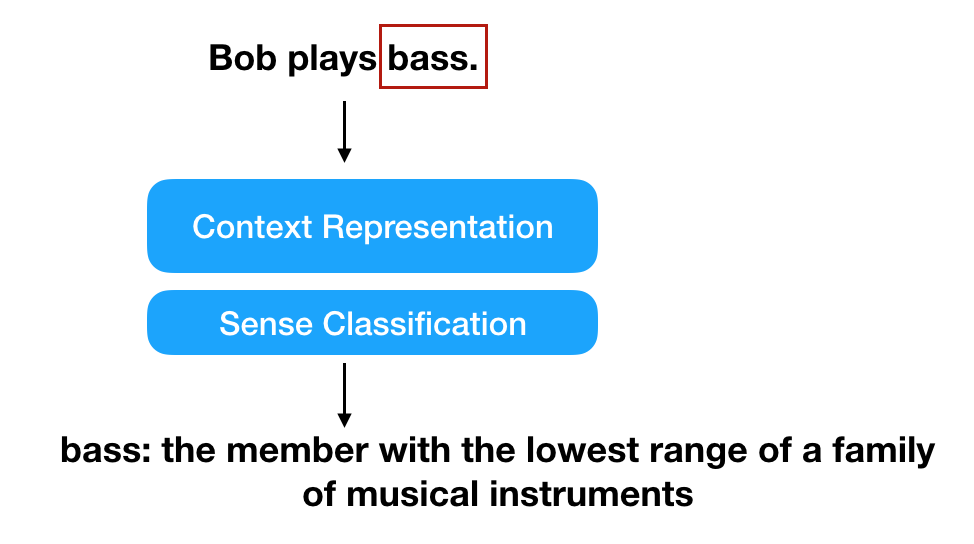
\includegraphics[width=0.7\textwidth]{graphs/overview.png}
\end{center}

We rely on Google to retrive information. The typical way we interact with
search engines is typing in search key words using natural languages. However
English words have different meanings in different contexts. A major challenge
to precisely retrive the desired information is for search engine to understand
the meaning of key words in a given context.

To solve this problem, we propose to build a word sense disambiguate system that
takes an English word and a sentence where it appears as input, and predicts the
sense of such word with regard to the given context. 

A pratical usage of our system, would be for the search engine to substitute the
key words with paraphases of the same predicted sense, thus it can retrive a
more complete set of results for a given user query.

\section{Related Work}

Major approaches to the word sense disambiguation problem can be briefly
categorized into three types: Knowledge-based, supervised learning, and
unsupervised learning. 

Knowledge based appraoch.
Lesk's algorithm~\cite{lesk1986automatic} is a
dictionary-based approach. It assumes that words appear within the same context
have related semantics. The alogrithm disambiguate word sense by finding the
dictionary definition that shares the most common words with the given context
sentence.

Supervised learning approaches. These approaches typically use a hand-annotated
Corpus as the training data set. The classifier is concerned on each individual
word, and the output is one of the definition of the ambiguous word in the
dictionary. Over the decades, people have proposed different algorithms to solve
this classification problem: decision-tree~\cite{quinlan1986induction}, 
Naive Bayers classifier~\cite{ng1997getting}, Neural
Network~\cite{cottrell1985connectionist}, and SVM~\cite{lee2002empirical}, etc.

Unsupervised approach. Such approaches~\cite{schutze1998automatic} assumes that
similar senses appear in similar contexts. By clustering occurrance of words
into clusters using some similarity measures, the sense of a new occurring word
can be induced by assigning it to the closest cluster.

% \textbf{Context representation.} To feed sentences into our system, we need to
% encode the context into some data structure. Previous researches have proposed
% several ways to represent context.

\section{Dataset}
We use Semcor~\cite{semcor} to generate our dataset.
Semcor is a Corpus that consist of a set of tagged sentences.
The tags provided with each word.
The tag information we used in this work includes: \\
(1) Word sense ID in WordNet~\cite{wordnet}, which is used as prediction label.\\
(2) Part-of-Speech tag. This is used to encode context.\\
(3) Lemma. This is used to remove the inflections of word form variations in
different contexts.\\ 
Specifically, in our work, we use lemma, instead of the word
itself, as the identifier for word occurrence counting.
However, in context representation, we use the original word.

Class imbalance is prevalent in ambiguous words.
Most words have some rare meanings with very few occurrences in the corpus.
This ends up minority class in the dataset: classes that only appears in a few
times (typicall less than ten times).

We discuss how we account for the class imbalance issues in our evaluation
(section~\ref{sec:eval:results}).

\section{Problem Formulation}

We formualte the word sense disambiguation task into a supervised multi-class
classification problem.
This problem can be represented as tuple $(X,Y,h)$, where $X$ is the instance
space, that contains the description of the object on which we are to predict, 
and $Y$ is the label space, from which each object draws a label,
and $h$ is the classification function $X \rightarrow Y$, that maps the
descriptoin of an object in instance space $X$ to label space $Y$.

Each targetted ambiguous word $w$ has it's own label space $Y_w$, and a shared
instance space $X$ with other ambiguous words.
Therefore, the solution to a word sense disambiguation is specific to each
individual ambiguous word.
For each ambigous word we train a specific classifier $h_w: X
\rightarrow Y_w$, that maps instance from $X$ to it's own label space $Y_w$.


\subsection{Data Preprocessing}

We use SemCor Corpus~\cite{semcor} to provide the raw data for human languages.
SemCor Corpus is a corpus where each word is tagged with a sense provided by
WordNet~\cite{wordnet}.
We then generate the dataset for this problem, in the following steps:

\begin{enumerate}
  \item Tokenization: transform the sentense strings into list of tokens
    (usually words).
  \item Part-of-Speech tagging: e.g. ``the/DT bar/NN was/VBD crowded/JJ'', where
    DT stands for Determiners, NN stands for Noun, etc.
  \item Lemmatization: e.g. $plays \rightarrow play$, $was \rightarrow be$.
  \item Feature extraction: select some features to represent the context.
\end{enumerate}

\Paragraph{Ambigous word}. 
Given an English word $w$, and a tagged corpus, we say the $w$ is ambiguous, if
it is tagged with at least two different WordNet Sense IDs in the corpus.

(1) Ambiguity: Multiple sense id occurences.
(2) Learnability: Enough overall occurences, and occurences for each sense ids.

\Paragraph{Context Representation}
We use Colocation~\cite{colocation} method to represent the context of a word.
For a given ambiguous word, we looks at the the preceding and succeeding words,
and their Part-of-Speech tags.
The size of the moving window can vary, we use two in this project, as suggested
by previous studies (CITE).
\begin{equation}
  [w_{i-2},POS_{i-2},w_{i-1},POS_{i-1},w_{i+1},POS_{i+1},w_{i+1},POS_{i+1}]
\end{equation}

Vector reprensetations.
Word2Vec(CITE)

\Paragraph{Construct training set for each target word}.
Let W be the set of English words that we want to do sense disambiguation. For
each $w \in W$, we need to extract a training set $X_w$ from the SemCor Corpus
as follow: 
\begin{enumerate}
  \item Draw a set of sentences $S_w$ from SemCor Corpus, where each 
$s \in S_w$ contains w. 
  \item Convert each sentence $s \in S_w$ to a feature vector x, and the sense
    label y. The set of all (x,y) pairs is our training set $X_w$.
\end{enumerate}

\subsection{Performance Measures}. 

For each target word, we partition the data into training set and test set. 
And evaluate classifiers on the training set using 0-1 loss.

\section{Model and Algorithms}

For this multi-class classification problem, we consider the following models,
using one-vs-all method to extend them to solve multi-class problem:

\Paragraph{Naive Bayes}

\Paragraph{Logistic Regression}


\Paragraph{Support Vector Machine}
\\We have built three types of SVM models for each target word: Linear SVM, RBF kernel SVM and Polynomial kernel SVM. For the purpose of multi-class classification task, we use the \texttt{svm.SVC()} method in \texttt{sklearn} module in Python. Specifically, we set the \texttt{kernel} attribute in \texttt{svm.SVC()} to be ``linear'', ``rbf'' and ``poly'' respectively for building the three types of SVM models.

For each type of SVM models, we execute a 3-fold cross-validation on the training set for choosing the best parameters. The \texttt{grid\_search.GridSearchCV()} method in \texttt{sklearn} module in Python is used for this. We maintain the default stratified 3-fold splitting approach during cross-validation. The parameter to be tuned for Linear SVM is C, for RBF SVM is \{C, gamma\}, and for Polynomial SVM is \{C, degree\}. The range of values for each parameter is set as follows.

C = [0.01, 0.1, 1, 10, 100] \\
gamma = [0.0001, 0.001, 0.01, 0.1, 1, 10] \\
degree = [2, 3, 4, 5]

Eventually, for each target word, each type of SVM models has its own tuned best parameters.


\Paragraph{Neural Network}
Since the feature contains the sentence structure, the model is designed to process having capability of recognize which word come first and later instead up allowing model randomly search the best combination. Causal convolution layer \ref{causal}, a type of convolution, has been used in this problem to maintain this time series like structure. In order to having a larger size of reception field, dilation blocks are used, in which each layer extract certain amount of feature with sequence information \ref{dilation}, so that it is quite possible to process a much longer sentence without changing the structure with additional information. Residual network structure \ref{res} has been used on dilation block to prevent gradient vanishing in deep network. \\
The overall model structure is a forward causal layer to process sentence in a forward sequence, followed by two dilation residual blocks. There is a parallel structure to process the sentence backward. Two dilation blocks skip connections on both sequence are concatenated, then into a fully connected layer and enters a Softmax layer to make classification prediction.

causal
van den Oord, Aaron, Kalchbrenner, Nal, and Kavukcuoglu, Koray. Pixel recurrent neural networks. ¨
arXiv preprint arXiv:1601.06759, 2016a.

dilation
Aaron van den Oord, Sander Dieleman, Heiga Zen, Karen Simonyan, Oriol Vinyals, Alex
Graves, Nal Kalchbrenner, Andrew Senior, and Koray Kavukcuoglu. Wavenet: A generative
model for raw audio. arXiv preprint arXiv:1609.03499, 2016.

res
He, Kaiming, Zhang, Xiangyu, Ren, Shaoqing, and Sun, Jian. Deep residual learning for image
recognition. CoRR, abs/1512.03385, 2015.

\textbf{Desired properties}. Since in our system design, we need to train a
classifier for each target word, the ideal method should have short training
time, and compact model representation.

\section{Experimental design and results}

\subsection{Dataset Selection}

There are morn than thousands of ambugious words in the SemCor corpuse, by our
definition in secton~\ref{sec:formulate:preprocess}, which will translate to
more than thousands of datasets and the corresponding machine learning tasks.
However, not all dataset is qualified for a tractable machine learning problem. 
The problem is that some words have senses that are rarely appeared in the
sencor corpus, which is typically 1 or 2 appearances.
The lack of data makes the word sense unlearnable.
Therefore, we use two criteria to select the set of training set we use in our
experiment:
(1) Overall instances greate than 200, 
and (2) Each sense ids (labels / classes) appear at least 20 times.

These critia filters out the eight words we use in evaluation
(section~\ref{sec:eval:results}).

\subsection{Parameters Tuning}

\Paragraph{Logistic Regression}
We first perform a parameter search over 5-fold cross-validation over the entire
training set for different words. We tested different regularization values,
solvers, multiclass metrics. Finally we found that in most cases by setting C=1,
solver=``newtown\_cg'', max\_iter = 500, and metric=``multinomial'' we can get
the best accuracy and f1 scores. We'll set them to be the global parameters over
logistic regression classifier for each word. 

\Paragraph{SVM}.
For each type of SVM models, we execute a 3-fold cross-validation on the
training set for choosing the best parameters. The
\texttt{grid\_search.GridSearchCV()} method in \texttt{sklearn} module in Python
is used for this. We maintain the default stratified 3-fold splitting approach
during cross-validation. The parameter to be tuned for Linear SVM is C, for RBF
SVM is \{C, gamma\}, and for Polynomial SVM is \{C, degree\}. The range of
values for each parameter is set as follows.

C = [0.01, 0.1, 1, 10, 100] \\
gamma = [0.0001, 0.001, 0.01, 0.1, 1, 10] \\
degree = [2, 3, 4, 5]

Eventually, for each target word, each type of SVM models has its own tuned best
parameters.

\Paragraph{Neural Network}.
Because the limitation of dataset and purpose of in comparison with other modeling method, the model parameters used in the network for comparison are two dilation blocks with each only two layers to process four words. Only forward processing blocks exist, since the dataset is too small, which has been under-fitting. Number of filters of both causal convolution and dilation layers is 8. Number of filters of dense layer before the softmax layer is 16. The data is trained the whole dataset of a word per batch, and repeated five times for the same dataset.

\subsection{Results}
\label{sec:eval:results}

We use \textbf{weighted} F1 scores to account for the class imbalance effect in
the dataset. 
That is, we first calculate F1 scores for each class, and then average them,
weighted by the number of each class in the test set.

\begin{figure}[h]
  \centering 
  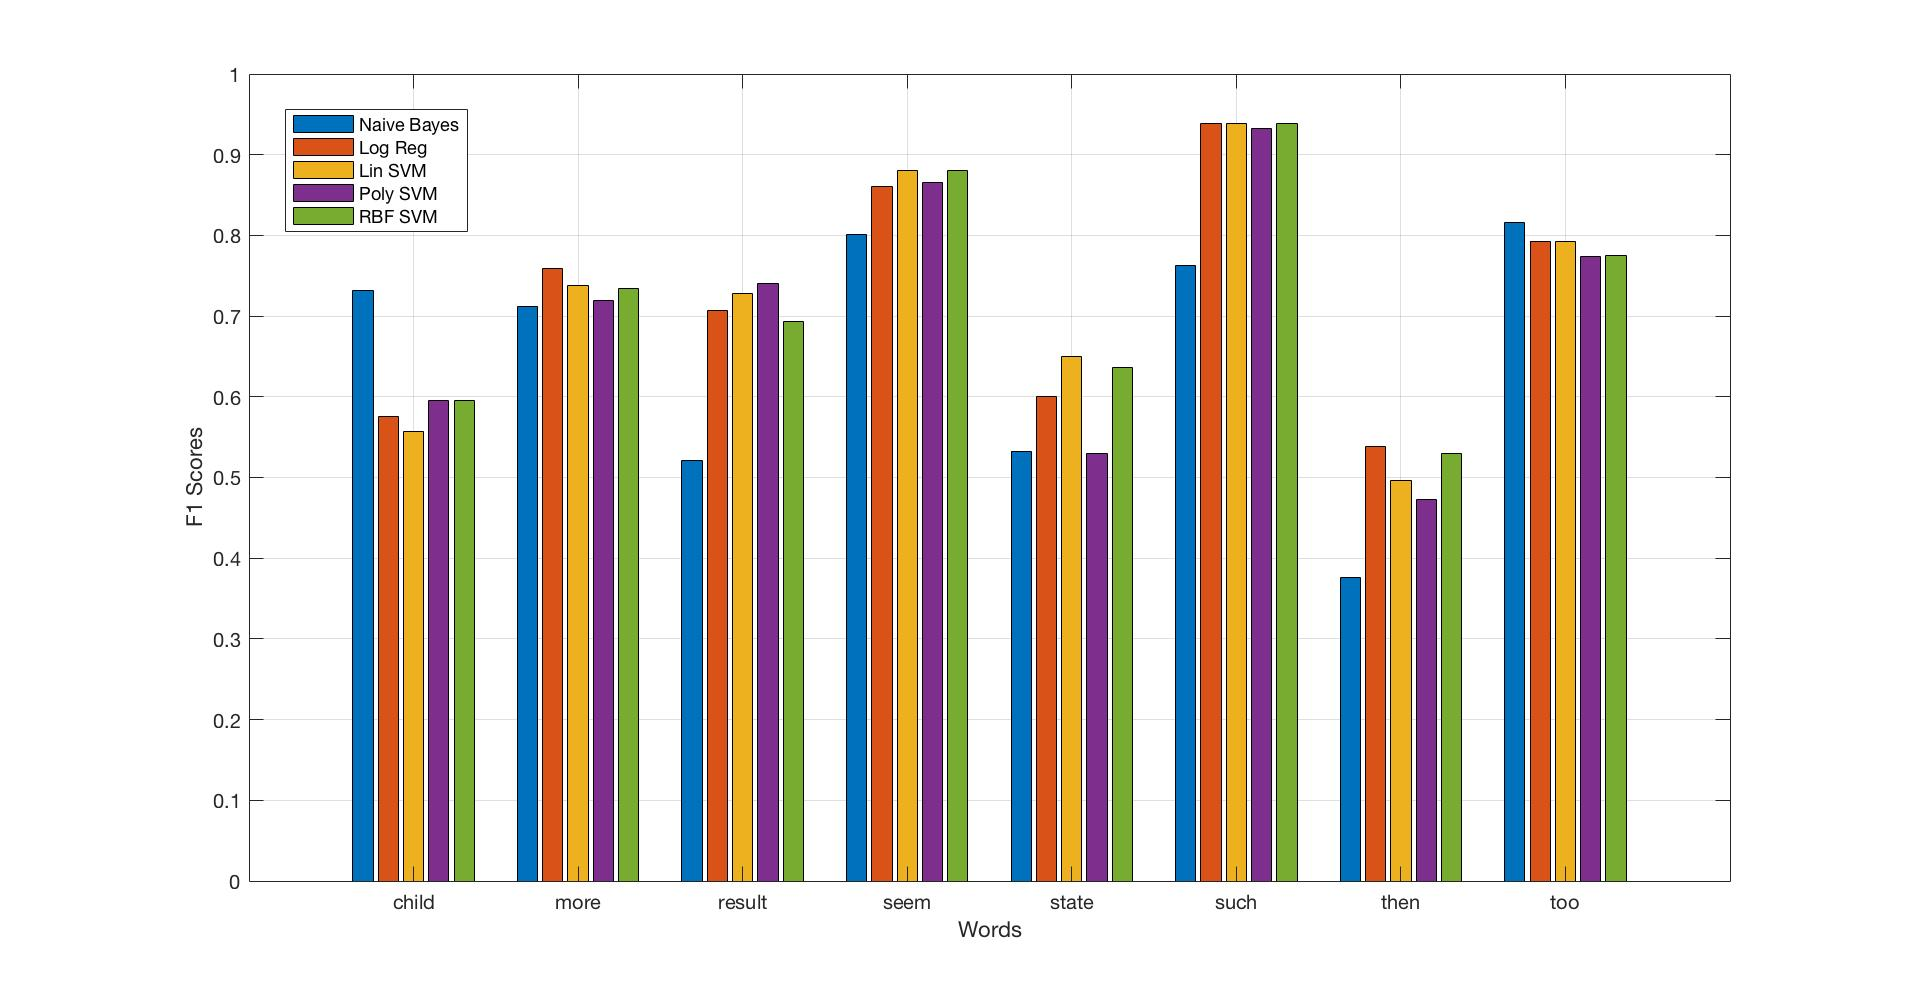
\includegraphics[width=0.7\textwidth]{plots/f1.jpg}
    \caption{Weighted F1 scores on each words}
    \label{fig:results:f1}
\end{figure}

Figure~\ref{fig:results:f1} shows the F1 socres for each classifer,
on each ambiguous word.

\Paragraph{Naive Bayes good at balanced classes}.
Naive Bayes shows high variance in terms of F1 score, compared to other
discriminative classifiers, as shown in figure~\ref{fig:results:f1}.
On word ``child'', Naive Bayes outperforms other discriminative classifiers by
about 16\%.
While on other words like ``result'', its F1 score is lowwer by about 28\%.
The problem is class imbalanced. 
On dataset of ``child'' has a class breakdown to (146,61), while words like
``result'' has a breakdown to (127,63,24).

\section{Conclusion}

We solve the word sense disambiguation problem using supervised learning
methods, 
We gather training data by generate feature instances and labels from
hand-tagged Corpus with word meaning defined by WordNet.
We evaluated multiple multi-class classification medels and algorithms on this
dataset, the result shows that Logistic Regression is the best all-around
algorithm to solve this word-sense classification problem, considering 
training time, model complexity, and the overall performance based on F1-score.

\Paragraph{Neural network underfit issue}. 
Because the dataset is very small, the simplified neural
network model remains severely underfit. More data is required to train the
model in order to improve the performance instead of adding more features into
the dataset. The network was originally designed for the whole sentence
processing, so as long as given a sufficient dataset, there is a huge potential
to give a better result. For future work, each dilation block could be replaced
by LSTM, which is also proven strong at time series type data processing. 


% \section{Plan of Work}
\begin{itemize}
  \item Week 1: Data preprocessing. 
      Tokenization: Haoxian Chen.
      Part-of-Speech tagging: Leshang Chen.
      Lemmanization: Hui Lyu.
      Feature extraction: Yanci Zhang.
  \item Week 2: Algorithm implementations.
      Naive Bayes: Haoxian Chen.
      Logistic Regression: Leshang Chen.
      Support Vector Machine: Hui Lyu.
      Nueral Network: Yanci Zhang.
  \item Week 3: Performance comparison and analysis. 
  \item Week 4: Report Writing.
\end{itemize}


% \section*{Acknowledgments}

%*********** Recommended section structure for project report below (comment out in project proposal) ************

%\section{Introduction}

%\section{Related Work}

%Note: Using BibTex makes it easy to include citations to references! For example, here are citations to Bishop's book \cite{Bishop06}, the UCI machine learning repository \cite{DuaKa17}, and a couple of papers \cite{FreundSc96,LeCun+15}.

%\section{Data Set}

%\section{Problem Formulation}

%\section{Algorithms}

%\section{Experimental Design and Results}

%\section{Conclusion and Discussion}

%\section*{Acknowledgments}


\newpage
%============================= BIBLIOGRAPHY ===============================

\bibliographystyle{unsrt}
\bibliography{bib}

\end{document}

%=========================== END DOCUMENT ==============================

